\documentclass[english]{article}

\usepackage[utf8]{inputenc}
\usepackage[T1]{fontenc}
\usepackage{babel}

\usepackage[linesnumbered,ruled,vlined]{algorithm2e}
\SetKw{KwNot}{not}
\SetKw{KwAnd}{and}
\SetKw{KwInIterate}{in}
\SetKw{KwBreak}{break}


\SetKwBlock{Init}{initialization}{}{}

\usepackage{amsfonts}
\usepackage{amsmath}

\setcounter{MaxMatrixCols}{20}

\usepackage{tikz}
\usetikzlibrary{calc}

\usepackage{xcolor}

\usepackage{subcaption}
\usepackage{lipsum}

\newcommand{\ruleB}{
    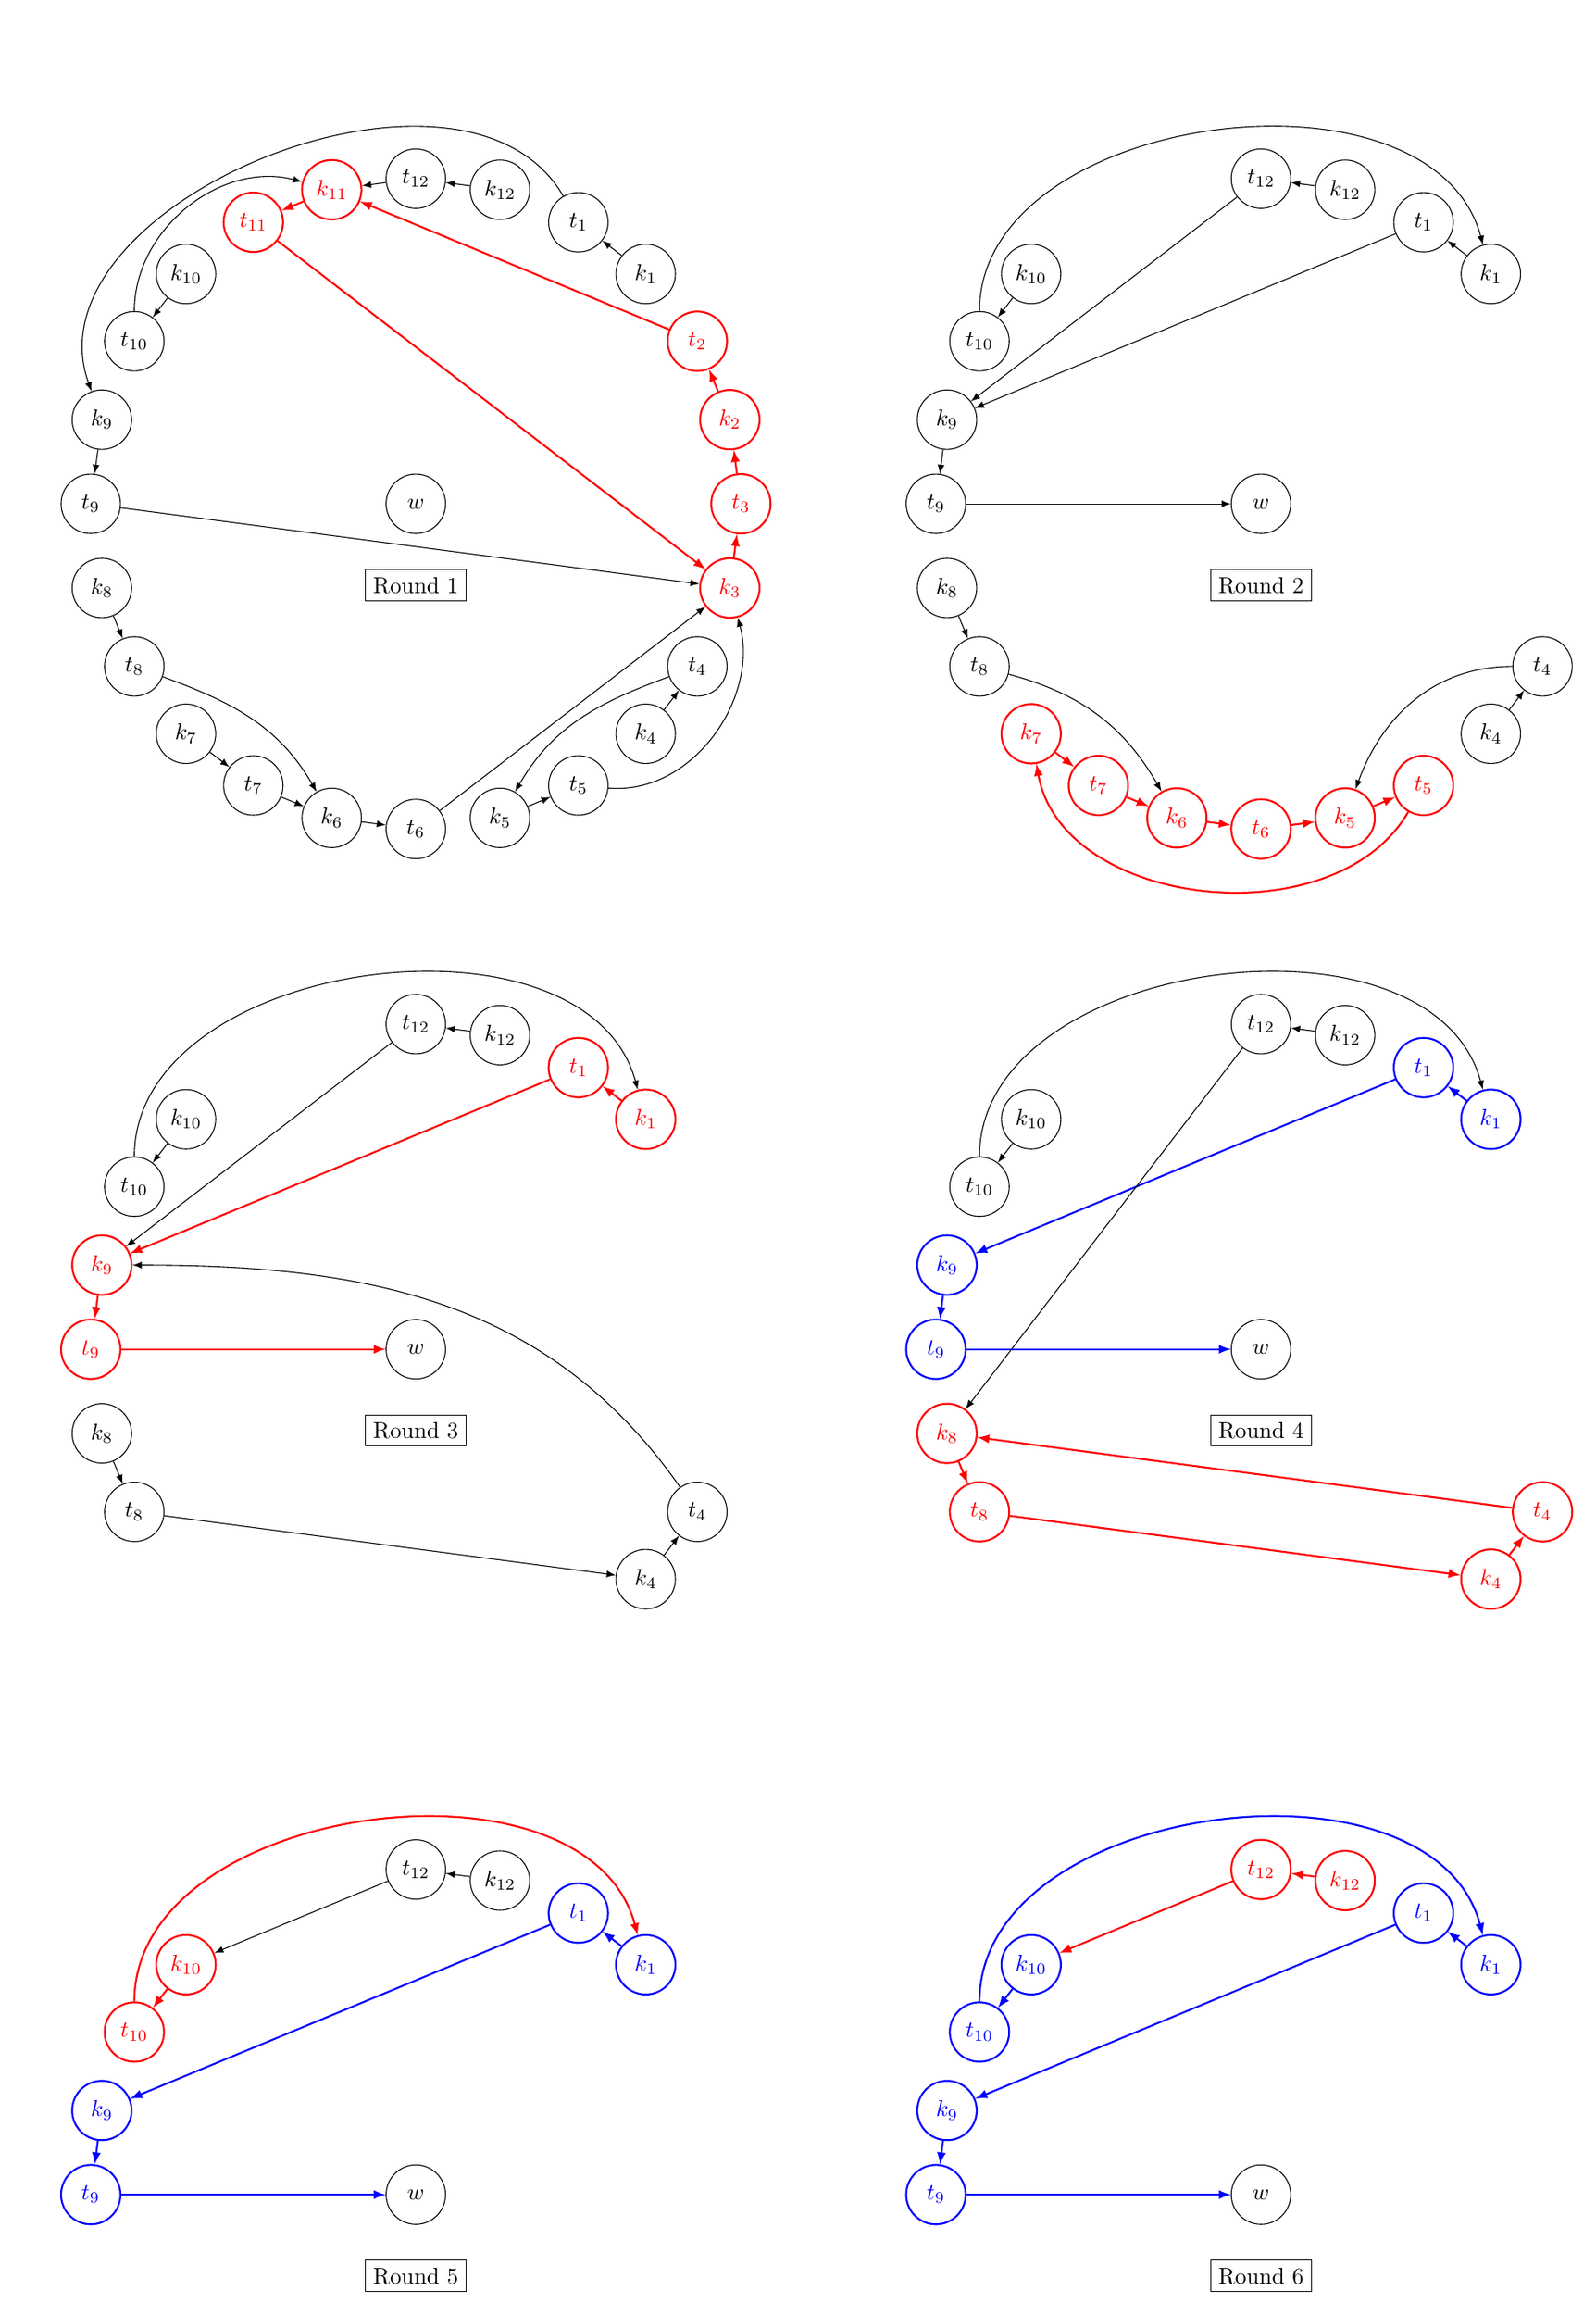
\begin{tikzpicture}[scale=5]

        \coordinate (b) at (2.6, 0);
        \coordinate (c) at (0,-2.6);
        \coordinate (d) at (2.6,-2.6);
        \coordinate (e) at (0,-5.2);
        \coordinate (f) at (2.6,-5.2);


        % \draw[->,>=latex, double] (1.15, 0) -- (1.45, 0);
        % \draw[->,>=latex, double] ($(b) + (225:1.15)$) -- ($(c) + (45:1.15)$);
        % \draw[->,>=latex, double] ($(c) + (0:1.15)$) -- ($(d) + (180:1.15)$);
        % \draw[->,>=latex, double] ($(d) + (270:1.15)$) -- ($(e) + (45:1.15)$);
        
        \node[draw] at (0,-0.25) {Round 1};
        \node[draw] at ($(b) + (0,-0.25)$) {Round 2};
        \node[draw] at ($(c) + (0,-0.25)$) {Round 3};
        \node[draw] at ($(d) + (0,-0.25)$) {Round 4};
        \node[draw] at ($(e) + (0,-0.25)$) {Round 5};
        \node[draw] at ($(f) + (0,-0.25)$) {Round 6};




        % Figure 1
        
        \node[draw, circle, minimum size=26pt] (w) at (0:0) {$w$};
        \node[draw, circle, minimum size=26pt] (t_1) at (60:1) {$t_1$};
        \node[draw, circle, minimum size=26pt] (k_1) at (45:1) {$k_1$};
        \node[draw, circle, minimum size=26pt, red, thick] (t_2) at (30:1) {$t_2$};
        \node[draw, circle, minimum size=26pt, red, thick] (k_2) at (15:1) {$k_2$};
        \node[draw, circle, minimum size=26pt, red, thick] (t_3) at (0:1) {$t_3$};
        \node[draw, circle, minimum size=26pt, red, thick] (k_3) at (345:1) {$k_3$};
        \node[draw, circle, minimum size=26pt] (t_4) at (330:1) {$t_4$};
        \node[draw, circle, minimum size=26pt] (k_4) at (315:1) {$k_4$};
        \node[draw, circle, minimum size=26pt] (t_5) at (300:1) {$t_5$};
        \node[draw, circle, minimum size=26pt] (k_5) at (285:1) {$k_5$};
        \node[draw, circle, minimum size=26pt] (t_6) at (270:1) {$t_6$};
        \node[draw, circle, minimum size=26pt] (k_6) at (255:1) {$k_6$};
        \node[draw, circle, minimum size=26pt] (t_7) at (240:1) {$t_7$};
        \node[draw, circle, minimum size=26pt] (k_7) at (225:1) {$k_7$};
        \node[draw, circle, minimum size=26pt] (t_8) at (210:1) {$t_8$};
        \node[draw, circle, minimum size=26pt] (k_8) at (195:1) {$k_8$};
        \node[draw, circle, minimum size=26pt] (t_9) at (180:1) {$t_9$};
        \node[draw, circle, minimum size=26pt] (k_9) at (165:1) {$k_9$};
        \node[draw, circle, minimum size=26pt] (t_10) at (150:1) {$t_{10}$};
        \node[draw, circle, minimum size=26pt] (k_10) at (135:1) {$k_{10}$};
        \node[draw, circle, minimum size=26pt, red, thick] (t_11) at (120:1) {$t_{11}$};
        \node[draw, circle, minimum size=26pt, red, thick] (k_11) at (105:1) {$k_{11}$};
        \node[draw, circle, minimum size=26pt] (t_12) at (90:1) {$t_{12}$};
        \node[draw, circle, minimum size=26pt] (k_12) at (75:1) {$k_{12}$};
    
        \draw[->,>=latex] (k_1) -- (t_1);
        \draw[->,>=latex, red, thick] (k_2) -- (t_2);
        \draw[->,>=latex, red, thick] (k_3) -- (t_3);
        \draw[->,>=latex] (k_4) -- (t_4);
        \draw[->,>=latex] (k_5) -- (t_5);
        \draw[->,>=latex] (k_6) -- (t_6);
        \draw[->,>=latex] (k_7) -- (t_7);
        \draw[->,>=latex] (k_8) -- (t_8);
        \draw[->,>=latex] (k_9) -- (t_9);
        \draw[->,>=latex] (k_10) -- (t_10);
        \draw[->,>=latex, red, thick] (k_11) -- (t_11);
        \draw[->,>=latex] (k_12) -- (t_12);
    
        \draw[->,>=latex] (t_1) [out=120, in=110] to (k_9);
        \draw[->,>=latex, red, thick] (t_2) to (k_11);
        \draw[->,>=latex, red, thick] (t_3) to (k_2);
        \draw[->,>=latex] (t_4) [out=200, in=60] to (k_5);
        \draw[->,>=latex] (t_5) [out=355, in = 285] to (k_3);
        \draw[->,>=latex] (t_6) to (k_3);
        \draw[->,>=latex] (t_7) to (k_6);
        \draw[->,>=latex] (t_8) [out=340, in=120] to (k_6);
        \draw[->,>=latex] (t_9) to (k_3);
        \draw[->,>=latex] (t_10) [out=90, in=165] to (k_11);
        \draw[->,>=latex, red, thick] (t_11) to (k_3);
        \draw[->,>=latex] (t_12) to (k_11);

        % Figure 2

        \node[draw, circle, minimum size=26pt] (w) at ($(b) + (0:0)$) {$w$};
        \node[draw, circle, minimum size=26pt] (t_1) at ($(b) + (60:1)$) {$t_1$};
        \node[draw, circle, minimum size=26pt] (k_1) at ($(b) + (45:1)$) {$k_1$};
        \node[draw, circle, minimum size=26pt] (t_4) at ($(b) + (330:1)$) {$t_4$};
        \node[draw, circle, minimum size=26pt] (k_4) at ($(b) + (315:1)$) {$k_4$};
        \node[draw, circle, minimum size=26pt, red, thick] (t_5) at ($(b) + (300:1)$) {$t_5$};
        \node[draw, circle, minimum size=26pt, red, thick] (k_5) at ($(b) + (285:1)$) {$k_5$};
        \node[draw, circle, minimum size=26pt, red, thick] (t_6) at ($(b) + (270:1)$) {$t_6$};
        \node[draw, circle, minimum size=26pt, red, thick] (k_6) at ($(b) + (255:1)$) {$k_6$};
        \node[draw, circle, minimum size=26pt, red, thick] (t_7) at ($(b) + (240:1)$) {$t_7$};
        \node[draw, circle, minimum size=26pt, red, thick] (k_7) at ($(b) + (225:1)$) {$k_7$};
        \node[draw, circle, minimum size=26pt] (t_8) at ($(b) + (210:1)$) {$t_8$};
        \node[draw, circle, minimum size=26pt] (k_8) at ($(b) + (195:1)$) {$k_8$};
        \node[draw, circle, minimum size=26pt] (t_9) at ($(b) + (180:1)$) {$t_9$};
        \node[draw, circle, minimum size=26pt] (k_9) at ($(b) + (165:1)$) {$k_9$};
        \node[draw, circle, minimum size=26pt] (t_10) at ($(b) + (150:1)$) {$t_{10}$};
        \node[draw, circle, minimum size=26pt] (k_10) at ($(b) + (135:1)$) {$k_{10}$};
        \node[draw, circle, minimum size=26pt] (t_12) at ($(b) + (90:1)$) {$t_{12}$};
        \node[draw, circle, minimum size=26pt] (k_12) at ($(b) + (75:1)$) {$k_{12}$};
    
        \draw[->,>=latex] (k_1) -- (t_1);
        \draw[->,>=latex] (k_4) -- (t_4);
        \draw[->,>=latex, red, thick] (k_5) -- (t_5);
        \draw[->,>=latex, red, thick] (k_6) -- (t_6);
        \draw[->,>=latex, red, thick] (k_7) -- (t_7);
        \draw[->,>=latex] (k_8) -- (t_8);
        \draw[->,>=latex] (k_9) -- (t_9);
        \draw[->,>=latex] (k_10) -- (t_10);
        \draw[->,>=latex] (k_12) -- (t_12);
    
        \draw[->,>=latex] (t_1) to (k_9);
        \draw[->,>=latex] (t_4) [out=180, in=70] to (k_5);
        \draw[->,>=latex, red, thick] (t_5) [out=240, in=280] to (k_7);
        \draw[->,>=latex, red, thick] (t_6) to (k_5);
        \draw[->,>=latex, red, thick] (t_7) to (k_6);
        \draw[->,>=latex] (t_8) [out=345, in=120] to (k_6);
        \draw[->,>=latex] (t_9) to (w);
        \draw[->,>=latex] (t_10) [out=90, in=105] to (k_1);
        \draw[->,>=latex] (t_12) to (k_9);
        
        % Figure 3

        \node[draw, circle, minimum size=26pt] (w) at ($(c) + (0:0)$) {$w$};
        \node[draw, circle, minimum size=26pt, red, thick] (t_1) at ($(c) + (60:1)$) {$t_1$};
        \node[draw, circle, minimum size=26pt, red, thick] (k_1) at ($(c) + (45:1)$) {$k_1$};
        \node[draw, circle, minimum size=26pt] (t_4) at ($(c) + (330:1)$) {$t_4$};
        \node[draw, circle, minimum size=26pt] (k_4) at ($(c) + (315:1)$) {$k_4$};
        \node[draw, circle, minimum size=26pt] (t_8) at ($(c) + (210:1)$) {$t_8$};
        \node[draw, circle, minimum size=26pt] (k_8) at ($(c) + (195:1)$) {$k_8$};
        \node[draw, circle, minimum size=26pt, red, thick] (t_9) at ($(c) + (180:1)$) {$t_9$};
        \node[draw, circle, minimum size=26pt, red, thick] (k_9) at ($(c) + (165:1)$) {$k_9$};
        \node[draw, circle, minimum size=26pt] (t_10) at ($(c) + (150:1)$) {$t_{10}$};
        \node[draw, circle, minimum size=26pt] (k_10) at ($(c) + (135:1)$) {$k_{10}$};
        \node[draw, circle, minimum size=26pt] (t_12) at ($(c) + (90:1)$) {$t_{12}$};
        \node[draw, circle, minimum size=26pt] (k_12) at ($(c) + (75:1)$) {$k_{12}$};
    
        \draw[->,>=latex, red, thick] (k_1) -- (t_1);
        \draw[->,>=latex] (k_4) -- (t_4);
        \draw[->,>=latex] (k_8) -- (t_8);
        \draw[->,>=latex, red, thick] (k_9) -- (t_9);
        \draw[->,>=latex] (k_10) -- (t_10);
        \draw[->,>=latex] (k_12) -- (t_12);
    
        \draw[->,>=latex, red, thick] (t_1) to (k_9);
        \draw[->,>=latex] (t_4) [out=125, in=0] to (k_9);
        \draw[->,>=latex] (t_8) to (k_4);
        \draw[->,>=latex, red, thick] (t_9) to (w);
        \draw[->,>=latex] (t_10) [out=90, in=105] to (k_1);
        \draw[->,>=latex] (t_12) to (k_9);

        % Figure 4
    
        \node[draw, circle, minimum size=26pt] (w) at ($(d) + (0:0)$) {$w$};
        \node[draw, circle, minimum size=26pt, blue, thick] (t_1) at ($(d) + (60:1)$) {$t_1$};
        \node[draw, circle, minimum size=26pt, blue, thick] (k_1) at ($(d) + (45:1)$) {$k_1$};
        \node[draw, circle, minimum size=26pt, red, thick] (t_4) at ($(d) + (330:1)$) {$t_4$};
        \node[draw, circle, minimum size=26pt, red, thick] (k_4) at ($(d) + (315:1)$) {$k_4$};
        \node[draw, circle, minimum size=26pt, red, thick] (t_8) at ($(d) + (210:1)$) {$t_8$};
        \node[draw, circle, minimum size=26pt, red, thick] (k_8) at ($(d) + (195:1)$) {$k_8$};
        \node[draw, circle, minimum size=26pt, blue, thick] (t_9) at ($(d) + (180:1)$) {$t_9$};
        \node[draw, circle, minimum size=26pt, blue, thick] (k_9) at ($(d) + (165:1)$) {$k_9$};
        \node[draw, circle, minimum size=26pt] (t_10) at ($(d) + (150:1)$) {$t_{10}$};
        \node[draw, circle, minimum size=26pt] (k_10) at ($(d) + (135:1)$) {$k_{10}$};
        \node[draw, circle, minimum size=26pt] (t_12) at ($(d) + (90:1)$) {$t_{12}$};
        \node[draw, circle, minimum size=26pt] (k_12) at ($(d) + (75:1)$) {$k_{12}$};
    
        \draw[->,>=latex, blue, thick] (k_1) -- (t_1);
        \draw[->,>=latex, red, thick] (k_4) -- (t_4);
        \draw[->,>=latex, red, thick] (k_8) -- (t_8);
        \draw[->,>=latex, blue, thick] (k_9) -- (t_9);
        \draw[->,>=latex] (k_10) -- (t_10);
        \draw[->,>=latex] (k_12) -- (t_12);
    
        \draw[->,>=latex, blue, thick] (t_1) to (k_9);
        \draw[->,>=latex, red, thick] (t_4) to (k_8);
        \draw[->,>=latex, red, thick] (t_8) to (k_4);
        \draw[->,>=latex, blue, thick] (t_9) to (w);
        \draw[->,>=latex] (t_10) [out=90, in=105] to (k_1);
        \draw[->,>=latex] (t_12) to (k_8);
        
        % figure 5

        \node[draw, circle, minimum size=26pt] (w) at ($(e) + (0:0)$) {$w$};
        \node[draw, circle, minimum size=26pt, blue, thick] (t_1) at ($(e) + (60:1)$) {$t_1$};
        \node[draw, circle, minimum size=26pt, blue, thick] (k_1) at ($(e) + (45:1)$) {$k_1$};
        \node[draw, circle, minimum size=26pt, blue, thick] (t_9) at ($(e) + (180:1)$) {$t_9$};
        \node[draw, circle, minimum size=26pt, blue, thick] (k_9) at ($(e) + (165:1)$) {$k_9$};
        \node[draw, circle, minimum size=26pt, red, thick] (t_10) at ($(e) + (150:1)$) {$t_{10}$};
        \node[draw, circle, minimum size=26pt, red, thick] (k_10) at ($(e) + (135:1)$) {$k_{10}$};
        \node[draw, circle, minimum size=26pt] (t_12) at ($(e) + (90:1)$) {$t_{12}$};
        \node[draw, circle, minimum size=26pt] (k_12) at ($(e) + (75:1)$) {$k_{12}$};
    
        \draw[->,>=latex, blue, thick] (k_1) -- (t_1);
        \draw[->,>=latex, blue, thick] (k_9) -- (t_9);
        \draw[->,>=latex, red, thick] (k_10) -- (t_10);
        \draw[->,>=latex] (k_12) -- (t_12);
    
        \draw[->,>=latex, blue, thick] (t_1) to (k_9);
        \draw[->,>=latex, blue, thick] (t_9) to (w);
        \draw[->,>=latex, red, thick] (t_10) [out=90, in=105] to (k_1);
        \draw[->,>=latex] (t_12) to (k_10);

        % figure 6

        \node[draw, circle, minimum size=26pt] (w) at ($(f) + (0:0)$) {$w$};
        \node[draw, circle, minimum size=26pt, blue, thick] (t_1) at ($(f) + (60:1)$) {$t_1$};
        \node[draw, circle, minimum size=26pt, blue, thick] (k_1) at ($(f) + (45:1)$) {$k_1$};
        \node[draw, circle, minimum size=26pt, blue, thick] (t_9) at ($(f) + (180:1)$) {$t_9$};
        \node[draw, circle, minimum size=26pt, blue, thick] (k_9) at ($(f) + (165:1)$) {$k_9$};
        \node[draw, circle, minimum size=26pt, blue, thick] (t_10) at ($(f) + (150:1)$) {$t_{10}$};
        \node[draw, circle, minimum size=26pt, blue, thick] (k_10) at ($(f) + (135:1)$) {$k_{10}$};
        \node[draw, circle, minimum size=26pt, red, thick] (t_12) at ($(f) + (90:1)$) {$t_{12}$};
        \node[draw, circle, minimum size=26pt, red, thick] (k_12) at ($(f) + (75:1)$) {$k_{12}$};
    
        \draw[->,>=latex, blue, thick] (k_1) -- (t_1);
        \draw[->,>=latex, blue, thick] (k_9) -- (t_9);
        \draw[->,>=latex, blue, thick] (k_10) -- (t_10);
        \draw[->,>=latex, red, thick] (k_12) -- (t_12);
    
        \draw[->,>=latex, blue, thick] (t_1) to (k_9);
        \draw[->,>=latex, blue, thick] (t_9) to (w);
        \draw[->,>=latex, blue, thick] (t_10) [out=90, in=105] to (k_1);
        \draw[->,>=latex, red, thick] (t_12) to (k_10);
    \end{tikzpicture}
}

\newcommand{\ruleA}{
    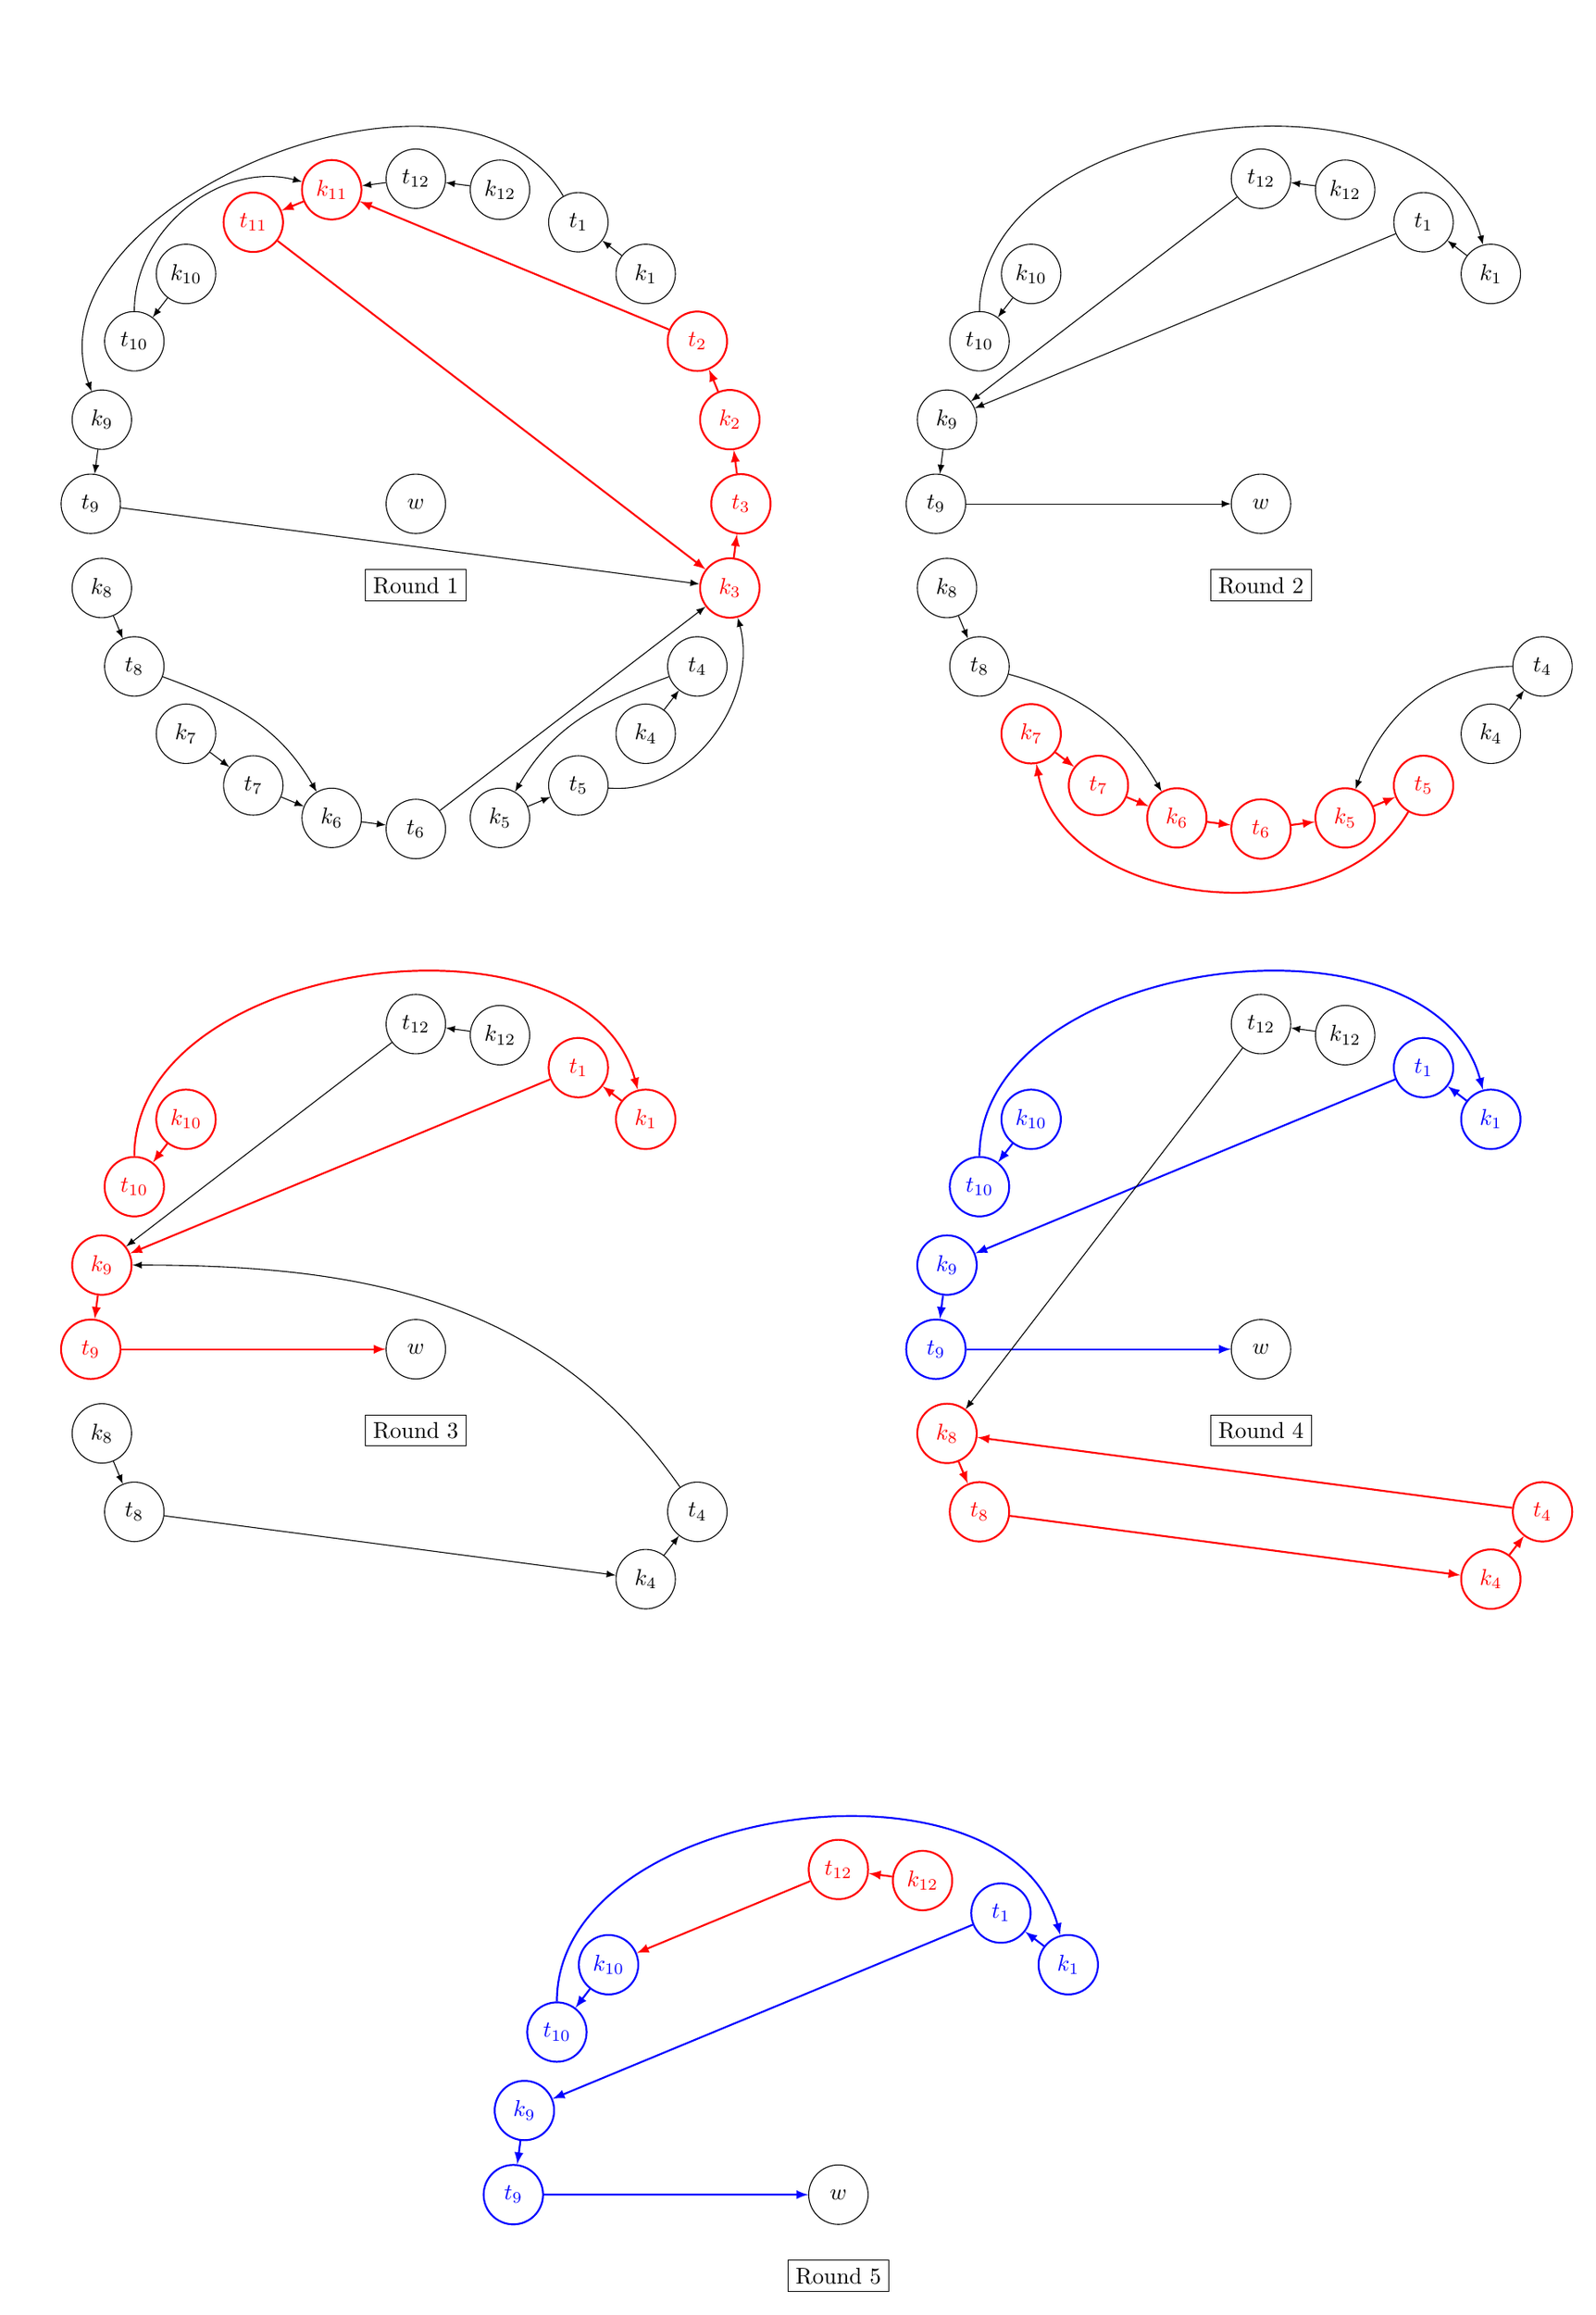
\begin{tikzpicture}[scale=5]

        \coordinate (b) at (2.6, 0);
        \coordinate (c) at (0,-2.6);
        \coordinate (d) at (2.6,-2.6);
        \coordinate (e) at (1.3,-5.2);

        % \draw[->,>=latex, double] (1.15, 0) -- (1.45, 0);
        % \draw[->,>=latex, double] ($(b) + (225:1.15)$) -- ($(c) + (45:1.15)$);
        % \draw[->,>=latex, double] ($(c) + (0:1.15)$) -- ($(d) + (180:1.15)$);
        % \draw[->,>=latex, double] ($(d) + (270:1.15)$) -- ($(e) + (45:1.15)$);
        
        \node[draw] at (0,-0.25) {Round 1};
        \node[draw] at ($(b) + (0,-0.25)$) {Round 2};
        \node[draw] at ($(c) + (0,-0.25)$) {Round 3};
        \node[draw] at ($(d) + (0,-0.25)$) {Round 4};
        \node[draw] at ($(e) + (0,-0.25)$) {Round 5};



        % Figure 1
        
        \node[draw, circle, minimum size=26pt] (w) at (0:0) {$w$};
        \node[draw, circle, minimum size=26pt] (t_1) at (60:1) {$t_1$};
        \node[draw, circle, minimum size=26pt] (k_1) at (45:1) {$k_1$};
        \node[draw, circle, minimum size=26pt, red, thick] (t_2) at (30:1) {$t_2$};
        \node[draw, circle, minimum size=26pt, red, thick] (k_2) at (15:1) {$k_2$};
        \node[draw, circle, minimum size=26pt, red, thick] (t_3) at (0:1) {$t_3$};
        \node[draw, circle, minimum size=26pt, red, thick] (k_3) at (345:1) {$k_3$};
        \node[draw, circle, minimum size=26pt] (t_4) at (330:1) {$t_4$};
        \node[draw, circle, minimum size=26pt] (k_4) at (315:1) {$k_4$};
        \node[draw, circle, minimum size=26pt] (t_5) at (300:1) {$t_5$};
        \node[draw, circle, minimum size=26pt] (k_5) at (285:1) {$k_5$};
        \node[draw, circle, minimum size=26pt] (t_6) at (270:1) {$t_6$};
        \node[draw, circle, minimum size=26pt] (k_6) at (255:1) {$k_6$};
        \node[draw, circle, minimum size=26pt] (t_7) at (240:1) {$t_7$};
        \node[draw, circle, minimum size=26pt] (k_7) at (225:1) {$k_7$};
        \node[draw, circle, minimum size=26pt] (t_8) at (210:1) {$t_8$};
        \node[draw, circle, minimum size=26pt] (k_8) at (195:1) {$k_8$};
        \node[draw, circle, minimum size=26pt] (t_9) at (180:1) {$t_9$};
        \node[draw, circle, minimum size=26pt] (k_9) at (165:1) {$k_9$};
        \node[draw, circle, minimum size=26pt] (t_10) at (150:1) {$t_{10}$};
        \node[draw, circle, minimum size=26pt] (k_10) at (135:1) {$k_{10}$};
        \node[draw, circle, minimum size=26pt, red, thick] (t_11) at (120:1) {$t_{11}$};
        \node[draw, circle, minimum size=26pt, red, thick] (k_11) at (105:1) {$k_{11}$};
        \node[draw, circle, minimum size=26pt] (t_12) at (90:1) {$t_{12}$};
        \node[draw, circle, minimum size=26pt] (k_12) at (75:1) {$k_{12}$};
    
        \draw[->,>=latex] (k_1) -- (t_1);
        \draw[->,>=latex, red, thick] (k_2) -- (t_2);
        \draw[->,>=latex, red, thick] (k_3) -- (t_3);
        \draw[->,>=latex] (k_4) -- (t_4);
        \draw[->,>=latex] (k_5) -- (t_5);
        \draw[->,>=latex] (k_6) -- (t_6);
        \draw[->,>=latex] (k_7) -- (t_7);
        \draw[->,>=latex] (k_8) -- (t_8);
        \draw[->,>=latex] (k_9) -- (t_9);
        \draw[->,>=latex] (k_10) -- (t_10);
        \draw[->,>=latex, red, thick] (k_11) -- (t_11);
        \draw[->,>=latex] (k_12) -- (t_12);
    
        \draw[->,>=latex] (t_1) [out=120, in=110] to (k_9);
        \draw[->,>=latex, red, thick] (t_2) to (k_11);
        \draw[->,>=latex, red, thick] (t_3) to (k_2);
        \draw[->,>=latex] (t_4) [out=200, in=60] to (k_5);
        \draw[->,>=latex] (t_5) [out=355, in = 285] to (k_3);
        \draw[->,>=latex] (t_6) to (k_3);
        \draw[->,>=latex] (t_7) to (k_6);
        \draw[->,>=latex] (t_8) [out=340, in=120] to (k_6);
        \draw[->,>=latex] (t_9) to (k_3);
        \draw[->,>=latex] (t_10) [out=90, in=165] to (k_11);
        \draw[->,>=latex, red, thick] (t_11) to (k_3);
        \draw[->,>=latex] (t_12) to (k_11);

        % Figure 2

        \node[draw, circle, minimum size=26pt] (w) at ($(b) + (0:0)$) {$w$};
        \node[draw, circle, minimum size=26pt] (t_1) at ($(b) + (60:1)$) {$t_1$};
        \node[draw, circle, minimum size=26pt] (k_1) at ($(b) + (45:1)$) {$k_1$};
        \node[draw, circle, minimum size=26pt] (t_4) at ($(b) + (330:1)$) {$t_4$};
        \node[draw, circle, minimum size=26pt] (k_4) at ($(b) + (315:1)$) {$k_4$};
        \node[draw, circle, minimum size=26pt, red, thick] (t_5) at ($(b) + (300:1)$) {$t_5$};
        \node[draw, circle, minimum size=26pt, red, thick] (k_5) at ($(b) + (285:1)$) {$k_5$};
        \node[draw, circle, minimum size=26pt, red, thick] (t_6) at ($(b) + (270:1)$) {$t_6$};
        \node[draw, circle, minimum size=26pt, red, thick] (k_6) at ($(b) + (255:1)$) {$k_6$};
        \node[draw, circle, minimum size=26pt, red, thick] (t_7) at ($(b) + (240:1)$) {$t_7$};
        \node[draw, circle, minimum size=26pt, red, thick] (k_7) at ($(b) + (225:1)$) {$k_7$};
        \node[draw, circle, minimum size=26pt] (t_8) at ($(b) + (210:1)$) {$t_8$};
        \node[draw, circle, minimum size=26pt] (k_8) at ($(b) + (195:1)$) {$k_8$};
        \node[draw, circle, minimum size=26pt] (t_9) at ($(b) + (180:1)$) {$t_9$};
        \node[draw, circle, minimum size=26pt] (k_9) at ($(b) + (165:1)$) {$k_9$};
        \node[draw, circle, minimum size=26pt] (t_10) at ($(b) + (150:1)$) {$t_{10}$};
        \node[draw, circle, minimum size=26pt] (k_10) at ($(b) + (135:1)$) {$k_{10}$};
        \node[draw, circle, minimum size=26pt] (t_12) at ($(b) + (90:1)$) {$t_{12}$};
        \node[draw, circle, minimum size=26pt] (k_12) at ($(b) + (75:1)$) {$k_{12}$};
    
        \draw[->,>=latex] (k_1) -- (t_1);
        \draw[->,>=latex] (k_4) -- (t_4);
        \draw[->,>=latex, red, thick] (k_5) -- (t_5);
        \draw[->,>=latex, red, thick] (k_6) -- (t_6);
        \draw[->,>=latex, red, thick] (k_7) -- (t_7);
        \draw[->,>=latex] (k_8) -- (t_8);
        \draw[->,>=latex] (k_9) -- (t_9);
        \draw[->,>=latex] (k_10) -- (t_10);
        \draw[->,>=latex] (k_12) -- (t_12);
    
        \draw[->,>=latex] (t_1) to (k_9);
        \draw[->,>=latex] (t_4) [out=180, in=70] to (k_5);
        \draw[->,>=latex, red, thick] (t_5) [out=240, in=280] to (k_7);
        \draw[->,>=latex, red, thick] (t_6) to (k_5);
        \draw[->,>=latex, red, thick] (t_7) to (k_6);
        \draw[->,>=latex] (t_8) [out=345, in=120] to (k_6);
        \draw[->,>=latex] (t_9) to (w);
        \draw[->,>=latex] (t_10) [out=90, in=105] to (k_1);
        \draw[->,>=latex] (t_12) to (k_9);
        
        % Figure 3

        \node[draw, circle, minimum size=26pt] (w) at ($(c) + (0:0)$) {$w$};
        \node[draw, circle, minimum size=26pt, red, thick] (t_1) at ($(c) + (60:1)$) {$t_1$};
        \node[draw, circle, minimum size=26pt, red, thick] (k_1) at ($(c) + (45:1)$) {$k_1$};
        \node[draw, circle, minimum size=26pt] (t_4) at ($(c) + (330:1)$) {$t_4$};
        \node[draw, circle, minimum size=26pt] (k_4) at ($(c) + (315:1)$) {$k_4$};
        \node[draw, circle, minimum size=26pt] (t_8) at ($(c) + (210:1)$) {$t_8$};
        \node[draw, circle, minimum size=26pt] (k_8) at ($(c) + (195:1)$) {$k_8$};
        \node[draw, circle, minimum size=26pt, red, thick] (t_9) at ($(c) + (180:1)$) {$t_9$};
        \node[draw, circle, minimum size=26pt, red, thick] (k_9) at ($(c) + (165:1)$) {$k_9$};
        \node[draw, circle, minimum size=26pt, red, thick] (t_10) at ($(c) + (150:1)$) {$t_{10}$};
        \node[draw, circle, minimum size=26pt, red, thick] (k_10) at ($(c) + (135:1)$) {$k_{10}$};
        \node[draw, circle, minimum size=26pt] (t_12) at ($(c) + (90:1)$) {$t_{12}$};
        \node[draw, circle, minimum size=26pt] (k_12) at ($(c) + (75:1)$) {$k_{12}$};
    
        \draw[->,>=latex, red, thick] (k_1) -- (t_1);
        \draw[->,>=latex] (k_4) -- (t_4);
        \draw[->,>=latex] (k_8) -- (t_8);
        \draw[->,>=latex, red, thick] (k_9) -- (t_9);
        \draw[->,>=latex, red, thick] (k_10) -- (t_10);
        \draw[->,>=latex] (k_12) -- (t_12);
    
        \draw[->,>=latex, red, thick] (t_1) to (k_9);
        \draw[->,>=latex] (t_4) [out=125, in=0] to (k_9);
        \draw[->,>=latex] (t_8) to (k_4);
        \draw[->,>=latex, red, thick] (t_9) to (w);
        \draw[->,>=latex, red, thick] (t_10) [out=90, in=105] to (k_1);
        \draw[->,>=latex] (t_12) to (k_9);

        % Figure 4
    
        \node[draw, circle, minimum size=26pt] (w) at ($(d) + (0:0)$) {$w$};
        \node[draw, circle, minimum size=26pt, blue, thick] (t_1) at ($(d) + (60:1)$) {$t_1$};
        \node[draw, circle, minimum size=26pt, blue, thick] (k_1) at ($(d) + (45:1)$) {$k_1$};
        \node[draw, circle, minimum size=26pt, red, thick] (t_4) at ($(d) + (330:1)$) {$t_4$};
        \node[draw, circle, minimum size=26pt, red, thick] (k_4) at ($(d) + (315:1)$) {$k_4$};
        \node[draw, circle, minimum size=26pt, red, thick] (t_8) at ($(d) + (210:1)$) {$t_8$};
        \node[draw, circle, minimum size=26pt, red, thick] (k_8) at ($(d) + (195:1)$) {$k_8$};
        \node[draw, circle, minimum size=26pt, blue, thick] (t_9) at ($(d) + (180:1)$) {$t_9$};
        \node[draw, circle, minimum size=26pt, blue, thick] (k_9) at ($(d) + (165:1)$) {$k_9$};
        \node[draw, circle, minimum size=26pt, blue, thick] (t_10) at ($(d) + (150:1)$) {$t_{10}$};
        \node[draw, circle, minimum size=26pt, blue, thick] (k_10) at ($(d) + (135:1)$) {$k_{10}$};
        \node[draw, circle, minimum size=26pt] (t_12) at ($(d) + (90:1)$) {$t_{12}$};
        \node[draw, circle, minimum size=26pt] (k_12) at ($(d) + (75:1)$) {$k_{12}$};
    
        \draw[->,>=latex, blue, thick] (k_1) -- (t_1);
        \draw[->,>=latex, red, thick] (k_4) -- (t_4);
        \draw[->,>=latex, red, thick] (k_8) -- (t_8);
        \draw[->,>=latex, blue, thick] (k_9) -- (t_9);
        \draw[->,>=latex, blue, thick] (k_10) -- (t_10);
        \draw[->,>=latex] (k_12) -- (t_12);
    
        \draw[->,>=latex, blue, thick] (t_1) to (k_9);
        \draw[->,>=latex, red, thick] (t_4) to (k_8);
        \draw[->,>=latex, red, thick] (t_8) to (k_4);
        \draw[->,>=latex, blue, thick] (t_9) to (w);
        \draw[->,>=latex, blue, thick] (t_10) [out=90, in=105] to (k_1);
        \draw[->,>=latex] (t_12) to (k_8);
        
        % figure 5

        \node[draw, circle, minimum size=26pt] (w) at ($(e) + (0:0)$) {$w$};
        \node[draw, circle, minimum size=26pt, blue, thick] (t_1) at ($(e) + (60:1)$) {$t_1$};
        \node[draw, circle, minimum size=26pt, blue, thick] (k_1) at ($(e) + (45:1)$) {$k_1$};
        \node[draw, circle, minimum size=26pt, blue, thick] (t_9) at ($(e) + (180:1)$) {$t_9$};
        \node[draw, circle, minimum size=26pt, blue, thick] (k_9) at ($(e) + (165:1)$) {$k_9$};
        \node[draw, circle, minimum size=26pt, blue, thick] (t_10) at ($(e) + (150:1)$) {$t_{10}$};
        \node[draw, circle, minimum size=26pt, blue, thick] (k_10) at ($(e) + (135:1)$) {$k_{10}$};
        \node[draw, circle, minimum size=26pt, red, thick] (t_12) at ($(e) + (90:1)$) {$t_{12}$};
        \node[draw, circle, minimum size=26pt, red, thick] (k_12) at ($(e) + (75:1)$) {$k_{12}$};
    
        \draw[->,>=latex, blue, thick] (k_1) -- (t_1);
        \draw[->,>=latex, blue, thick] (k_9) -- (t_9);
        \draw[->,>=latex, blue, thick] (k_10) -- (t_10);
        \draw[->,>=latex, red, thick] (k_12) -- (t_12);
    
        \draw[->,>=latex, blue, thick] (t_1) to (k_9);
        \draw[->,>=latex, blue, thick] (t_9) to (w);
        \draw[->,>=latex, blue, thick] (t_10) [out=90, in=105] to (k_1);
        \draw[->,>=latex, red, thick] (t_12) to (k_10);
    \end{tikzpicture}
}

\newcommand{\N}{\mathbb{N}}

\newtheorem{lemm}{Lemma}

\title{Matching mechanisms for kidney transplantations}
\author{Tristan François}

\begin{document}

\maketitle

\section{Two Simple Approaches}

\subsection*{Question 1}

\begin{algorithm}[H]
% \DontPrintSemicolon
\caption{Direct Donation}

\KwIn{A number $n$ of patient and, for all patients $i \in \N$, their set of compatible donors $K_i \subseteq [\![1, n]\!]$.}
\KwOut{A set of pairs donor-patient pairs $M$ and a waiting list $w$.}
\Init{
    $M = \emptyset$\;
    $w = []$\;
}
\Begin{
\For{$i = 1$ \KwTo $n$}{
    \If{$k_i \in K_i$}{
        $M = M \cup \{(k_i,t_i)\}$\; 
    }
    \Else{
        $w$.add($t_i$)
    }
}
\Return{$c$, $w$}}

\end{algorithm}

The implementation in python is pretty straightforward. The python function takes as parameter an integer $n$ and an integer set array of size $n$. The use of python set allows to test the if condition in constant times. The only difference with pseudo-code is the use of a list rather than a set for the variable c. This choice was made to avoid the unnecessary heaviness of the set data structure, but does not change the complexity.

\subsection*{Question 2}

Our matching algorithm must prioritize the patients with the highest priority. It must also ensure that all patients will leave with a donor that suited them better than their paired donor and the waiting list, otherwise some patients may not participate in the exchange program.

Our greedy algorithm therefore consists of browsing the patients in descending order of priority and matching them to their preferred donor whose paired patient does not prefer the waiting list or his donor to the donor of the priority patient. Note that a patient can be matched to his own donor.

\begin{algorithm}[H]
    % \DontPrintSemicolon
    \caption{Greedy Matching}
    
    \KwIn{A number $n$ of patient, a strict priority list of the patients U and, for all patients $i \in \N$, their set of compatible donors $K_i \subseteq [\![1, n]\!]$ and their strict preference relation $P_i$ over $K_i \cup \{k_i, w\}$. The priority list is an integer list that starts with the index of the highest priority patient and goes to the index of the lowest priority patient.}
    \KwOut{A matching $M$.}

    \Init{
    $M = \emptyset$\;
    $is\_matched = Boolean[1..n]$\;
    $sorted\_K = IntegerList[1..n]$\;
    %\tcc{Initialize arrays}
    \For{$i = 1$ \KwTo $n$}{
        is\_matched[i] = False\;
        %\tcc{The sort function returns a list of the elements of $K\_i$ sorted in descending order according to the preference relation $P\_i$.}
        sorted\_K[i] = sort($K_i$, $P_i$) \tcp*{\textcolor{red}{$\mathcal{O}(n\log(n))$}}
    }
    }

    \Begin{
    
    \tcc{Iterate over all patient by decreasing priority}
    \For{ $u \in U$}{
        \If{\KwNot $is\_matched[u]$}{
            \For{$v \in sorted\_K[u]$}{
                \If{\KwNot $is\_matched[v]$}{
                    \tcc{If $t_v$ prefer $k_u$ over $k_v$ and $w$}
                    \If{$k_v \, P_v \, k_u$ \KwAnd $k_v \, P_v \, w$}{
                        $M = M \cup \{((k_u, t_v), (k_v, t_u))\}$\;
                        is\_matched[u] = True\;
                        is\_matched[v] = True\;
                        \KwBreak \;
                    }
                }
            }
        }
    }
    \Return{M}
    }
    
\end{algorithm}

We start by initializing an $is\_matched$ array to keep track of which pair has already been matched and an integer list array $sorted\_K$ that contains, for each patient of index $i$, the indexes of the preferred donors in descending order of preference. The sort function returns a list of the elements of $K_i$ sorted in descending order according to the preference relation $P_i$.

The implementation is almost exactly the pseudo-code.

\section{Efficient stategy-proof exchange mechanism}

\subsection*{Question 3}

Let $(k_1,t_1)$ be a pair of donor-patient and assume there is no cycle. Consider the chain starting from $(k_1,t_1)$. Since there is a finite number $n$ of donor-patient pairs and there is no cycle, the chain cannot be infinite. Finally, since the only way for a chain to stop is that $w$ belong to the chain, $(k_1,t_1)$ is indeed a tail of a $w$-chain.

Thus either there exists a cycle, or each pair is the tail of some $w$-chain.

\subsection*{Question 4}

The general sequence of the algorithm is shown in the algorithm below. For the sake of brevity, we omit some auxiliary functions like \texttt{GetCycles}, which returns the cycles in a directed graph, or \texttt{Update}, which updates the state of the graph according to the procedure described in the project description. The others not detailed functions will be discussed after the algorithm and the pseudo-code of \texttt{SelectChainA} is given in algorithm \ref{ccaux}.

\begin{algorithm}[H]
    \SetKwFunction{AssChain}{AssignChain}
    \SetKwFunction{AssCycle}{AssignCycle}
    \SetKwFunction{GetCycles}{GetCycles}
    \SetKwFunction{SelectChainA}{SelectChainA}
    \SetKwFunction{Update}{Update}

    % \DontPrintSemicolon
    \caption{Cycles and Chains Matching Algorithm}
    
    \KwIn{A number $n$ of patient, a strict priority list of the patients $U$ and, for all patients $i \in \N$, their set of compatible donors $K_i \subseteq [\![1, n]\!]$, their strict preference relation $P_i$ over $K_i \cup \{k_i, w\}$ and the initial graph $G$.}
    \KwOut{A matching $M$.}

    \Init{
    $M = \emptyset$\;
    $removed = \emptyset$\;
    $passive = \emptyset$\;
    $unavailable = \emptyset$\;
    }

    \Begin{
    
    \While{$|removed| + |passive| \neq n$}{
        cycles = \GetCycles{G}\;
        \If{$|cycles| \neq 0$}{
            \For{$cycle \in cycles$}{
                \AssCycle{cycle}\tcp*{modifies $M$ and $removed$}
            }
        }
        \Else{
            chain = \SelectChainA{G}\;
            \tcc{modifies $M$, $passive$ and $unavailable$}
            \AssChain{chain}\;
        }
        \Update{G}\;
    }
    \Return{M}
    }
    
\end{algorithm}

At any time, we keep up to date the $ removed $ set of vertices removed from the graph during the cycle deletion, the $ passive $ set of vertices which are still in the graph but whose target no longer changes, as well as the $ unavailable $ set of vertices to which we can no longer point. Those sets allow to update the graph without difficulty. Each time we choose a $w$-chain, all of its vertices are added to $ passive $ and all vertices except the head are added to $ unavailable $. These operations are performed by the \texttt{AssignCycle} and \texttt{AssignChain} functions. 

We still have to discuss a crucial part of the algorithm, the chain selection rule A. According to the rule statement, the first thing to do is find the longest chains.

In order to quickly obtain the longest chains, it should be noted that the transposed graph is a tree with root $ w $. A depth-first search gives us the depth of all vertices in the tree. Once the depths are obtained, it is very easy to find the longest chains. This is what the omitted \texttt{GetLongestChains} function does.

Once we have the longest chains, we still need to find the one with the patient with the highest priority. For this, we take all the patients who appear in the longest chains, and we sort them in decreasing order of priority. Then, we iterate on this patient list, look to which chain the patient belongs to, and remove all the other chains. When there's only one chain left, we've found the one we're interested in.

\begin{algorithm*}[H]
    \label{ccaux}
    \SetKwFunction{AssChain}{AssignedChain}
    \SetKwFunction{AssCycle}{AssignedCycle}
    \SetKwFunction{GetCycles}{GetCycles}
    \SetKwFunction{GetLongestChains}{GetLongestChains}
    \SetKwFunction{SelectChainA}{SelectChainA}
    \SetKwFunction{Update}{Update}

    \SetKwProg{Fn}{Function}{:}{}


    % \DontPrintSemicolon
    \caption{Chain Selection Rule A}

    \Fn{\SelectChainA{}}{
        chains = \GetLongestChains{}\;
        $nodes = \emptyset$\;
        \For{$chain \in chains$}{
            $nodes = nodes \cup chain$ 
        }
        \For{$node \in nodes$ by decreasing priority}{
            $new\_chains = \emptyset$\;
            \For{$chain \in chains$}{
                \If{$node \in chain$}{
                    $new\_chains = new\_chains \cup chain$ \;
                }
            }
            \If{$|new\_chains| = 1$}{
                \Return{$new\_chains.pop()$}\;
            }
            \ElseIf{$|new\_chains| > 1$}{
                chains = new\_chains\;
            }
        }
    }
    
\end{algorithm*}

For the implementation, readability was preferred over pure efficiency, which is why an object structure with heavy use of python set was preferred. The use of python set is also due to the fact that we often have to test the membership of an element in a set, whether for the construction of the graph, in the cycle search, or in the selection of the chain.
To make things a bit simpler, we can notice that, since a donor always points to his paired patient, there is no need to have a separate node for the donor and the patient. Thus in the implementation, there is only one node in the graph for each donor-patient pair.

\subsection*{Question 5}

Let's run the Cycles and Chains Matching Algorithm with rule A on this example. Graphs associated with every round are shown in figure \ref{fig:ruleA}.

The initial graph contains a cycle $C_1 = (k_3, t_3, k_2, t_2, k_{11}, t_{11})$. The first round of the algorithm therefore consists in detecting this cycle, assigning the kidneys to the patients and then eliminating the cycle.

After removing the first circle, a new circle $C_2 = (k_5, t_5, k_7, t_7, k_6, t_6)$ is formed. In the second round, this cycle is therefore deleted.

At the start of the third round, there is no more circle. The graph contains longest $w$-chains : $W_1 = (k_8, t_8, k_4, t_4, k_9, t_9)$ and $W_2 = (k_{10}, t_{10}, k_1, t_1, k_9, t_9)$. Since the highest priority patient $ t_1 $ is only present in $W_2$,  $W_2$ is chosen. The kidneys are assigned and the chain remains in the graph for the next round but patients pointing to other kidneys than $k_10$ in the chain are redirected.

After the redirect, a new circle $ C_3 = (k_4, t_4, k_8, t_8)$ has formed. The fourth round therefore consists in the elimination of this cycle.

There is no new circle and the patient $ t_{12} $ now points to $ k_{10} $ forming a chain of maximum length $ W_3 = (k_{12}, t_{12}, k_{10}, t_{10}, k_1, t_1, k_9, t_9) $. Round 5 assigns kidneys $ k_{10} $ to patient $ t_{12} $ and there are no more patients with no kidneys. The algorithm stops.

The final matching is:
\begin{equation*}
\left(
\begin{matrix}
    t_1 & t_2 & t_3 & t_4 & t_5 & t_6 & t_7 & t_8 & t_9 & t_{10} & t_{11} & t_{12} \\
    k_9 & k_{11} & k_2 & k_8 & k_7 & k_5 & k_6 & k_4 & w & k_1 & k_3 & k_{10}
\end{matrix}
\right)
\end{equation*}

\newpage

\begin{figure}[!ht]
    \centering
    \scalebox{0.5}{\ruleA}
    \caption{State of the graph at every round.}
    \label{fig:ruleA}
\end{figure}

\newpage 
\subsection*{Question 6}

If the selection rule keep in the procedure any selected $w$-chain at a non-terminal round, then every unasigned kidney is available at every round of the procedure. Therefore, at every round of the algorithm, a patient can only be assigned to his best choice among remaining kidneys. The only way to give him a better kidney is to take it back from a patient whose assignement occurs in a previous round. Since this patient had his best choice at the time, he will strictly disprefer the new matching. Thus, the exchange mechanism is efficient.

\subsection*{Question 7}

If we swap $k_8$ and $k_9$ in the order of preference of the twelfth patient, then in round 3 the longest $w$-chain becomes $(k_{12}, t_{12}, k_8, t_8, k_4, t_4, k_9, t_9)$ and $t_{12}$ is assigned to $k_8$, which he strictly prefers to $k_{10}$, that he would get by being honest about his preferences. Therefore the exchange mechanism with chain selection rule A is not strategy-proof.

\subsection*{Question 8}

The first two rounds are the same as with rule A. In the third round, we choose the $w$-chain starting with $(k_1, t_1)$, the highest priority pair. As with rule A, during the fourth round we delete the cycle $(k_4, t_4, k_8, t_8)$. Finally, on round 5 and 6, pairs $(k_{10}, t_{10})$ then $(k_{12}, t_{12})$ come to lengthen the chain formed in the third round. The final matching is the same as the one obtained with rule A.

Graphs associated with every round are shown in figure \ref{fig:ruleB}.

\newpage

\begin{figure}[!ht]
    \centering
    \scalebox{0.5}{\ruleB}
    \caption{Problem Graph at the beginning of each round.}
    \label{fig:ruleB}
\end{figure}

In agreement with Theorem 2, we can notice that agents cannot hope to get a better assignment by lying about their preferences. For example, the strategy used in the previous question by the twelfth patient is no longer effective, because whatever his preferences, he will be affected last.

\section{Integer programming formulation}

\subsection*{Question 9}

In order to list all the minimal infeasible paths, we will simply use a recursive function \texttt{Aux} which, given a graph $G$, a vertex $v$ and an integer $k$, returns all the paths of lengths $k+1$ starting at $v$. In order to avoid cycles, we add an $inpath$ variable, a set containing the vertices already in the current path. Finally, we called this function on all the vertices of the graph.

\begin{algorithm}
    \SetKwFunction{Faux}{Aux}
    \SetKwProg{Fn}{Function}{:}{}

    \caption{Minimal infeasible paths}
    
    \KwIn{$G = (V, E)$ a graph and $k$ the threshold.}
    \KwOut{The set of all minimal infeasible paths.}

    \Begin{
        $paths = \emptyset$\;
        \For{$v \in V$}{
            $paths = paths \cup \{\Faux(G, v, k, \emptyset)\}$\;
        }
        \Return{paths}\;
    }

    \tcc{Return the list of all minimal infeasible path starting from $v$}
    
    \Fn{\Faux{G, v, k, inpath}}{
        \If{$k = 0$}{
            \Return{$\{[v]\}$}\;
        }
        $inpath = inpath \cup \{v\}$\;
        $paths = \emptyset$\;
        \For{$neighbour \in v.neighbours$}{
            \If{$neighbour \notin inpath$}{
                \For{$path \in \Faux(G, neighbour, k-1, inpath)$}{
                    $paths = paths \cup \{path.add\_first(v)\}$\;
                }
            }
        }
        $inpath = inpath \setminus \{v\}$\;
        \Return{paths}\;
    }
\end{algorithm}

The implementation in python is very similar to the pseudo-code, except that the algorithm returns a list of paths rather than a set. The graph is given in the form of adjacency lists, in order to be able to iterate quickly on the neighbors.

\begin{figure}[ht]
    \centering
    \begin{tabular}{|c|c|c|c|c|}
        \hline
        file & CPU time & $|V|$ & $|E|$ & number of paths \\
        \hline
        test2.txt & $0.097 * 10^{-3}$ seconds & 12 & 18 & 45 \\
        test3.txt & $31.008 * 10^{-3}$ seconds & 17 & 229 & 28188 \\
        \hline
    \end{tabular}
    \caption{Mean execution time over 1000 iterations on an Intel i5-6200U processor.}
\end{figure}

\subsection*{Question 10}

Let $n$ be the number of patients and $M$ the adjacency matrix of the graph. We will denote by $ m_ {i, j} $ the coefficients of $M$. We therefore have $m_{i, j} = 1$ if the kidney $k_i$ is compatible with
the patient $t_j$ and $m_{i, j} = 0$ otherwise. We also define $\Pi$ as the set of minimal infeasible paths. 

For all $(i, j) \in {[\![1, n]\!]}^2$, we define a variable $a_{i,j}$ which is equal to $1$ if the kidney $k_i$ is assigned to the patient $t_j$ and equal to $0$ otherwise. We denote by A the assignment matrix whose coefficients are $a_{i, j}$. Since we are trying to maximize the number of transplants, our objective function will be:
\begin{equation}\label{obj_func}
    \max_{A} \sum_{(i, j) \in {[\![1, n]\!]}^2} a_{i,j}
\end{equation}
However, we are subject to a few of constraints. To begin with, by definition of $a_{i, j}$, we have the following first set of constraints.
\begin{equation}\label{cons1}
    \forall (i, j) \in {[\![1, n]\!]}^2, \; a_{i,j} \in \{0, 1\}
\end{equation}
In addition a kidney $ k_i $ can only be assigned to a patient $ t_j $ if $ t_j $ is compatible with $ k_i $, in other words $ a_{i,j} $ cannot be equal to $1$ if $ m_{i,j} $ is $0$. Therefore $ a_{i,j} $ is necessarily less than or equal to $ m_{i,j} $. So we have a new set of constraints:
\begin{equation}\label{cons2}
    \forall (i, j) \in {[\![1, n]\!]}^2, \; a_{i,j} \leq m_{i,j}
\end{equation}
In addition, a patient cannot receive more than 1 kidney and a donor will not donate his kidney if his paired patient does not receive a kidney. Thus, we have:
\begin{equation}\label{cons3}
    \forall j \in [\![1, n]\!], \; \sum_{i = 1}^{n} a_{i,j} \leq 1\\
\end{equation}
\begin{equation}\label{cons4}
    \forall j \in [\![1, n]\!], \; \sum_{i = 1}^{n} a_{j,i} \leq \sum_{i = 1}^{n} a_{i,j}
\end{equation}
Finally, we need to verify that there is no exchange cycle of length more than the threshold $K$. To do this, it suffices to check that none of the minimal infeasible paths is taken. We thus obtain our last set of constraints:
\begin{equation}\label{cons5}
    \forall \{i_1, i_2, \dots, i_{K+1} \} \in \Pi, \; \sum_{k = 1}^{K} a_{i_k,i_{k+1}} \leq K - 1
\end{equation}
Our integer linear program is therefore the maximization of \ref{obj_func} subject to \ref{cons1}, \ref{cons2}, \ref{cons3}, \ref{cons4} and \ref{cons5}.

\subsection*{Question 11}

The relaxed problem is the same as before with constraint \ref{cons1} replaced by a new constraint:
\begin{equation}\label{cons6}
    \forall (i, j) \in {[\![1, n]\!]}^2, \; 0 \leq a_{i,j} \leq 1
\end{equation}
In the following algorithm, we assume given a function allowing to solve a linear program and returning the solution and the value of the objective function. If the problem is infeasible, the value of the objective function will be $ - \infty $. We also assume given a function that test if the solution is an integer one. 

At each node of the tree, we will force a variable $ a_{i, j} $ to take the value 0 on one branch and 1 on the other by adding the constraints $ a_{i, j} \leq 0 $ and $ a_{i, j} \geq 1 $, then we'll take the best solution of the two branches.
\begin{algorithm}
    \SetKwFunction{Faux}{BranchAndBound}
    \SetKwFunction{IsInt}{IsIntegerSolution}
    \SetKwProg{Fn}{Function}{:}{}

    \caption{Branch and Bound}
    
    \KwIn{A linear problem $prob$ and a set of relaxed variables $vars$}
    \KwOut{A solution to the problem}

    \Begin{
        \Return{\Faux{prob, vars, 0, $\emptyset$}}
    }

    % \tcc{Return the list of all minimal infeasible path starting from $v$}
    
    \Fn{\Faux{prob, vars, best, solution}}{
        score, new\_sol = prob.solve()\;
        \If{$score = -\infty$}{
            \Return{best, solution}\;
        }
        \ElseIf{$score < best$}{
            \Return{best, solution}\;
        }
        \ElseIf{\IsInt{new\_solution}}{
            \Return{score, new\_sol}\;
        }
        \Else{
            x = vars.pop()\;
            prob.add\_constraint($x \geq 1$)\;
            $score_1$, $new\_sol_1$ = \Faux{prob, vars, best, solution}\;
            prob.remove\_constraint($x \geq 1$)\;
            prob.add\_constraint($x \leq 0$)\;
            $score_2$, $new\_sol_2$ = \Faux{prob, vars, best, solution}\;
            prob.remove\_constraint($x \leq 0$)\;
            vars.add(x)\;
            \If{$score_1 > score_2$}{
                \Return{$score_1$, $new\_sol_1$}\;
            }
            \Else{
                \Return{$score_2$, $new\_sol_2$}\;
            }

        }
    }
\end{algorithm}

For the implementation, we used the Python \texttt{Pulp} library as the linear program solver. Unfortunately, it is not possible to simply remove a constraint from a linear problem with this library. Instead of the problem, we therefore pass the variables, the objective function and the list of constraints to each recursive call and we recreate the problem each time. Other than that, the implementation is very similar to pseudo-code.

\subsection*{Question 12}

The results of the previous algorithm are available in the following figure. Note that the execution time is very good because, in both cases, the relaxed problem directly gives an entire solution. The Branch-and-Bound algorithm is therefore unnecessary for the cases below. However, there are cases where the linear program does not give integer solutions. The code provided with the report contains functions capable of generating such cases.

\begin{figure}[ht]
    \centering
    \begin{tabular}{|c|c|c|c|}
        \hline
        file & CPU time & selected cycles & objective value \\
        \hline
        test2.txt & 0.041 seconds & 
        \begin{tabular}{@{}c@{}} $(0, 8, 2)$, $(1, 10, 9)$, \\ $(3, 4, 5)$\end{tabular}
        & 9 \\
        \hline
        test3.txt & 1.658 seconds & 
        \begin{tabular}{@{}c@{}} $(0, 1, 14)$, $(2, 6)$, $(3)$, \\ $(4)$, $(5)$, $(7)$, $(8, 16)$, \\ $(9, 10)$, $(11)$, $(12)$, $(13)$, $(15)$  \end{tabular}
        & 17 \\
        \hline
    \end{tabular}
    \caption{Results and mean execution time over 10 iterations on an Intel i5-6200U processor.}
\end{figure}

\subsection*{Question 13}

\end{document}